\chapter{Methodology}\label{Sec:Methodology}

\section{Computational Implementation}

The simulations were performed using Python, on a Macbook Air with a 1.1 GHz Quad-Core Intel Core i5 processor and 8GB RAM. The Hamiltonian (Eq. \ref{Eq:BHM}) was expressed as a matrix in a basis of Fock states of the system. For one particle, these basis states are $b_i^{\dag}|0\rangle$ for all sites $i$; and for two particles, $b_i^{\dag}b_j^{\dag}|0\rangle$ for all pairs of (different) sites $ij$, and $\frac{1}{\sqrt{2}}(b_i^{\dag})^2|0\rangle$ when both particles occupy site $i$. The state of the system is represented by a vector $\textbf{c}$ of the coefficients $c_\alpha$ of the basis states $|\alpha\rangle$ in the expansion of $|\Psi\rangle$:
\begin{subequations}
    \begin{equation}
        |\Psi\rangle = \sum_{\alpha}c_\alpha |\alpha\rangle
    \end{equation}
    \begin{equation}
        c_\alpha = \langle \alpha|\Psi \rangle
    \end{equation}
\end{subequations}
Both periodic (illustrated in Fig. \ref{Fig:Lattice_Enumerated}) and open boundary conditions were implemented. Except where stated otherwise, the results throughout this report are for periodic systems, which are generally less susceptible to finite-size effects. 

\section{Evaluating Time-Evolution}

Time-evolution of the quantum state was calculated using one of two methods:

\begin{enumerate}
    \item The eigenstate method: the Hamiltonian is fully diagonalized to obtain the eigenvalues $\{\epsilon_n\}$ and eigenstates $\{|\phi_n\rangle\}$. $|\Psi(t')\rangle$ is calculated by expanding $|\Psi(t)\rangle$ in terms of $\{|\phi_n\rangle\}$:
    \begin{equation}\label{Eq:EigenstateEvolution}
        |\psi(t')\rangle = \sum_n \exp{\left(-\frac{i\epsilon_{n}(t'-t)}{\hbar}\right)}\langle \phi_n|\psi(t)\rangle|\phi_n\rangle
    \end{equation}
    \item The propagator method: the time-evolution is calculated with the exponential of the Hamiltonian:
    \begin{equation}\label{Eq:PropagatorEvolution}
        |\psi(t')\rangle = \exp{\left(-\frac{iH(t'-t)}{\hbar}\right)}|\psi(t)\rangle
    \end{equation}
    using matrix exponentiation functions. For convenience, $\hbar$ was set to 1 throughout the project. Eq. \ref{Eq:EigenstateEvolution} can be derived from Eq. \ref{Eq:PropagatorEvolution} by inserting the resolution of the identity $\mathbbm{1}=\sum_n|\phi_n\rangle\langle\phi_n|$. 
\end{enumerate}

The specific choice of algorithms and their computation times are presented in Appendix \ref{App:Timing}. The propagator method, whose computation time scales favourably as $\mathcal{O}(N)$ with the number of basis states $N$, was predominantly used; the eigenstate method was occasionally preferable with large values of $U$ or long simulation times. 

Occasionally throughout the project, only a partial diagonalization of the Hamiltonian was required; for example, to obtain the eigenspectrum of the doublon band (Section \ref{Sec:Doublon_Eigenspectrum}). Here, the Hamiltonian was expressed as a sparse matrix and the Lanczos algorithm \cite{Weisse}, which is able to rapidly find a subset of the eigenvalues (though not fully diagonalize the Hamiltonian), was used.

\vspace{0.5cm}

\begin{figure}[ht]
    \centering
    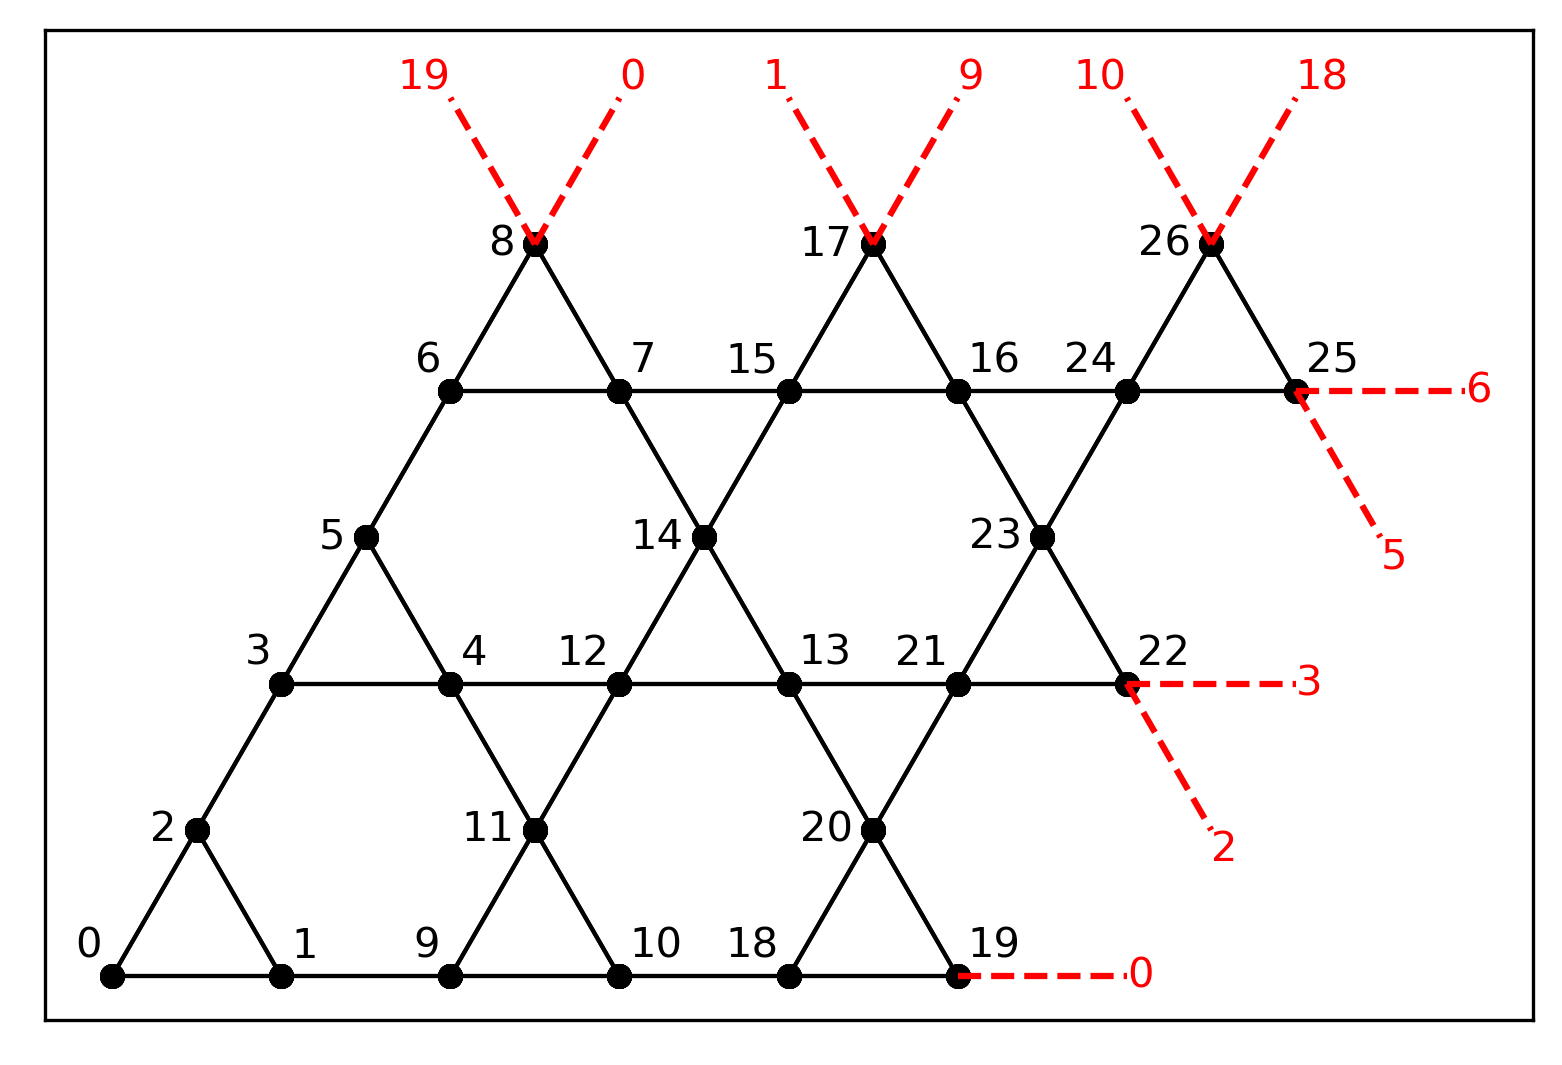
\includegraphics[width=10cm]{Figures/Lattice_Enumerated}
    \caption{Kagome lattice, with sites indexed and periodic boundary conditions illustrated.}
    \label{Fig:Lattice_Enumerated}
\end{figure}